\documentclass[11pt]{article}
\usepackage[margin=1in]{geometry}
\usepackage{amsmath,amssymb}
\usepackage{lmodern}
\usepackage[T1]{fontenc}
\usepackage{enumitem}
\usepackage{microtype}
\usepackage{tikz}
\usetikzlibrary{arrows.meta,angles,quotes,calc,decorations.pathreplacing}

\title{2025 F=ma Exam Review}
\author{Nathan P.}
\date{February 8, 2026}

\begin{document}
\maketitle

\section*{Problem 2}
It’s a good idea to form the triangle to determine that disk 2 and 3 would have $v\cos 30^\circ$.
Set up momentum and energy conservation and solve the system; the sign of $v_f$ is direction-sensitive.

\begin{center}
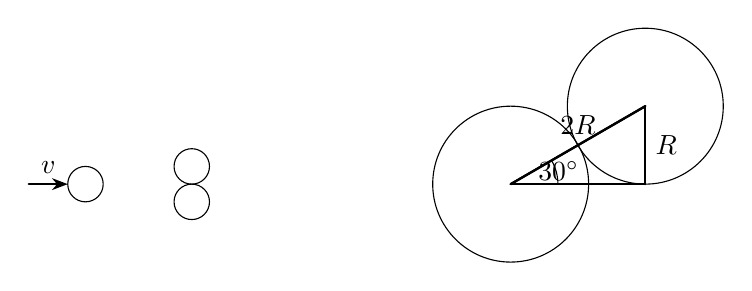
\begin{tikzpicture}[scale=0.9, line cap=round, line join=round, >={Stealth[length=2mm]}]
  % Incoming disk with velocity arrow (same size as the two stacked disks)
  \draw (-1.0,0) circle (0.25);
  \draw[->,thick] (-1.8,0) -- (-1.25,0) node[midway,above] {$v$};

  % Two stacked disks (touching each other, and the incoming one is tangent to the top disk)
  \draw (0.5,0.25) circle (0.25);
  \draw (0.5,-0.25) circle (0.25);

  % Contact geometry sketch (two disks and a line of centers)
  % Make the two large circles bigger and tangent (not overlapping)
  \coordinate (A) at (5.0,0);
  \coordinate (B) at (6.9,1.10);
  \draw (A) circle (1.10);
  \draw (B) circle (1.10);
  \draw[thick] (A) -- (B);
  % Larger right triangle for the 30-degree label
  \coordinate (C) at (6.9,0);
  \draw[thick] (A) -- (C);
  \draw[thick] (C) -- (B);
  \pic[draw, "$30^\circ$", angle radius=6mm, angle eccentricity=1.05] {angle = C--A--B};
  \draw[thick] (A) -- (B) node[midway, above] {$2R$};
  \draw[thick] (C) -- (B) node[midway, right] {$R$};
\end{tikzpicture}
\end{center}

\section*{Problem 3}
Key idea: it’s colliding with equal masses, so it will transfer all its momentum in the component parallel to the line of action of its impulse while keeping the perpendicular/tangential component.
Draw it out.

\section*{Problem 4}
It’s like circular motion. Use the definition of acceleration and some small-angle vector approximations: $s=r\,d\theta$ and $\omega=v/r$.
\[
a=\frac{dv}{dt}=\frac{du}{dt}=u_2\frac{d\theta}{dt}=u_2\omega=\frac{u_1u_2}{L},
\qquad
\omega=\frac{u_1}{L}.
\]

\begin{center}
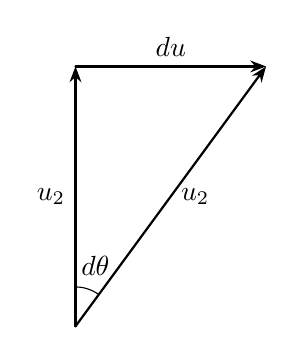
\begin{tikzpicture}[scale=1.1, line cap=round, line join=round, >={Stealth[length=2mm]}]
  % Vectors: u2 (left), u2 (right), du (top), and the small angle d\theta
  \coordinate (O) at (0,0);
  \coordinate (A) at (0,3.0);
  \coordinate (B) at (2.2,3.0);

  % Left u2
  \draw[->,thick] (O) -- (A) node[midway, left] {$u_2$};

  % Top du
  \draw[->,thick] (A) -- (B) node[midway, above] {$du$};

  % Right u2 (tilted)
  \draw[->,thick] (O) -- (B) node[midway, right] {$u_2$};

  % Angle label d\theta at the origin between OA and OB
  \pic[draw, angle radius=5mm] {angle = B--O--A};
  \node at (0.23,0.7) {$d\theta$};
\end{tikzpicture}
\end{center}

\section*{Problem 5}
Write out all force equations; solve for $N_1$, $N_2$, $f_1$, and $f_2$.
Since $f\le \mu N$, we have $\mu \le f/N$.

\section*{Problem 6}
Write it out and make sure to distinguish the height drop on the ramp and the height of the fall.
The fall time $t=\sqrt{2h/g}$ is constant because the height of fall is constant.
The horizontal velocity when shooting off the ramp is proportional to the square root of the height drop on the ramp: $v=\sqrt{2gh}$, and $x=vt$.
So $2.5x$ means $2.5v$, which means $6.25h$ (height drop on the ramp).

\section*{Problem 7}
\[
K_1+K_2+U_g+U_s.
\]
Rule out B and D because you don’t subtract energy.
Rule out E because if $\theta_1$ and $\theta_2$ were the same then it’d be
\[
\tfrac12 m\ell^2\omega^2 + \tfrac12 m(2\ell\omega)^2
=\tfrac52 m\ell^2\omega^2,
\]
which is greater than the $\tfrac12+\tfrac12$ $m\ell^2\omega^2$ in option E.
Option C makes sense for being $\theta_1-\theta_2$ because if $\theta$ was $45^\circ$ that should maximize $K$, not make the term disappear.

Anyways, the real way to do it is $K=K_1+K_2$. Get $K_2$ with $\tfrac12 mv_2^2$ and $v_2=v_1+v_{\mathrm{rel}}$, and $v_{\mathrm{rel}}$ is just $\ell\omega_2$.
So $v_2^2$ is the dot product of $v_1+v_{\mathrm{rel}}$ with itself:
\[
v_2^2=v_1^2+\ell^2\omega_2^2+2v_1(\ell\omega_2)\cos(\theta_1-\theta_2).
\]

\section*{Problem 9}
If you imagine the position vector $\mathbf{r}$ from $C_1$ to $C_2$ and from $C_2$ to $C_3$ and so on, they all spin at $\omega$, so it’ll just be a straight line spinning at $\omega$.
Don’t be fooled by the answer options; make your own judgment and recognize the simplicity they’re testing in these complex-looking dynamics problems.

\begin{center}
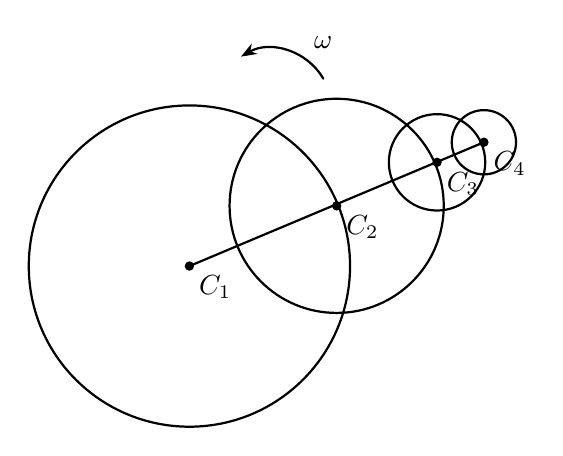
\begin{tikzpicture}[scale=0.85, line cap=round, line join=round, >={Stealth[length=2mm]}]
  % Centers C1..C4
  \coordinate (C1) at (0,0);
  \coordinate (C2) at (2.2,0.9);
  \coordinate (C3) at (3.7,1.55);
  \coordinate (C4) at (4.4,1.85);

  % Overlapping circles getting progressively smaller
  \draw[thick] (C1) circle (2.4);
  \draw[thick] (C2) circle (1.6);
  \draw[thick] (C3) circle (0.72);
  \draw[thick] (C4) circle (0.48);

  % One straight line connecting the centers (shows they rotate together)
  \draw[thick] (C1) -- (C4);

  % Dots at centers
  \fill (C1) circle (2pt);
  \fill (C2) circle (2pt);
  \fill (C3) circle (2pt);
  \fill (C4) circle (2pt);

  % Labels
  \node[below right] at (C1) {$C_1$};
  \node[below right] at (C2) {$C_2$};
  \node[below right] at (C3) {$C_3$};
  \node[below right] at (C4) {$C_4$};

  % Single omega indicating shared rotation
  \draw[->,thick] (2.0,2.8) arc[start angle=30, end angle=120, radius=0.9];
  \node[above] at (2,3.1) {$\omega$};
\end{tikzpicture}
\end{center}

\section*{Problem 12}
My mistake was being too hasty and writing $0.5$ for 50 grams instead of $0.05$. Be careful with numbers.
When correcting, I mistakenly put $I=\tfrac12 mr^2$ when for point masses it’s just $I=mr^2$.
Otherwise this was a simple momentum conservation question.
You could also just have used linear momentum because they are point masses.

\section*{Problem 14}
It’s good to recognize that it’d be harder to get a shell rolling, so that would stop slipping later.
My mistake was thinking mass affected acceleration: $\mu mg=ma$, so $m$ cancels.
Frictional $a$ is independent of mass while $\alpha$ depends on rotational inertia.


\section*{Problem 16}
Pressure is inversely proportional to radius: $\Delta P \propto 1/R$.
The smaller the bubble, the higher the pressure.

\section*{Problem 17}
The fact that it’s negative means the conservative force pushes it outward (the graph is a hill); regular springs have positive $U$.
You can treat $x$ and $y$ directions as independent.
$x^2+y^2(=r^2)$ means it’s pushed radially outward.
The force is growing, so the trajectory will approach a line.

\section*{Problem 18}
$x$ depends on $y$ because they are multiplied.
``Some direction'' must be $y=x$ so that $kxy/2=kx^2/2$, so it’s stable.
Pushing $\ell$ in the direction $y=x$ would have $x=\ell/\sqrt{2}$ and $y=\ell/\sqrt{2}$, so $xy=\ell^2/2$.
So $U=k(\ell^2/2)/2$, so $k_{\mathrm{eff}}=k/2$.

\begin{center}
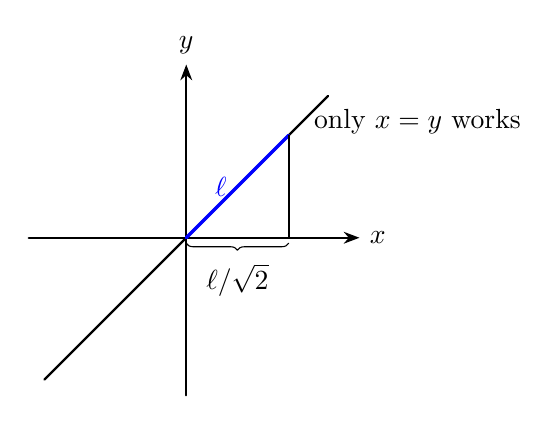
\begin{tikzpicture}[scale=1.0, line cap=round, line join=round, >={Stealth[length=2mm]}]
  % Axes
  \draw[->,thick] (-2,0) -- (2.2,0) node[right] {$x$};
  \draw[->,thick] (0,-2) -- (0,2.2) node[above] {$y$};

  % Line y=x
  \draw[thick] (-1.8,-1.8) -- (1.8,1.8);
  \node[above right] at (1.5,1.2) {$\text{only } x=y \text{ works}$};

  % Displacement vector of length \ell along y=x
  \coordinate (O) at (0,0);
  \coordinate (P) at (1.3,1.3);
  \draw[very thick, blue] (O) -- (P) node[midway, left] {$\ell$};

  % Projection on x-axis: \ell/\sqrt{2}
  \draw[thick] (P) -- (1.3,0);
  \draw[decorate, decoration={brace, mirror, raise=2pt}] (0,0) -- (1.3,0)
    node[midway, below=6pt] {$\ell/\sqrt{2}$};
\end{tikzpicture}
\end{center}

\section*{Problem 19}
$P\propto E\propto mv^2$, $m\propto v \text{ (continuity)}$, and given $v\propto h$: $2h$ means $2v$ means $8P$.

\section*{Problem 20}
Giving it a radial velocity affects $a$ and $T$ negligibly.

\section*{Problem 21}
It’s a good idea to use the continuity equation. Careful: the question asks for the difference in the speeds.

\section*{Problem 22}
\[
P_1+\tfrac12\rho v_1^2=P_2+\tfrac12\rho v_2^2,
\qquad
\Delta P=P_1-P_2=\rho g\,\Delta h.
\]
Solve for $\Delta h$.

\section*{Problem 23}
Find an expression for the variable you’re measuring, then find relative uncertainties.
If a measurement has ``smallest divisions'' at some unit, the uncertainty is half that unit.
If you take two measurements, $\Delta x$ is the average of the difference of the measurements, while the relative uncertainty is $\Delta x$ divided by the average of the measurements.
Once you see $\Delta g/g$ is negligible, don’t even bother calculating it.

\section*{Problem 25}
Given $M\gg m$, it is an inertial frame traveling at constant velocity, so doing physics in that frame works.
We can conserve energy to get that $m$ ends up with $\sqrt{2gh}$ in that frame; back in the lab frame we add the prism’s $v=\sqrt{2gh}$, so the total is $2\sqrt{2gh}$.

\end{document}
